\section{Results}\label{sec:results}

\subsection{Point-forecast sanity}

Table~\ref{tab:e0} verifies the fixed forecasting layer is not degraded:
the online pool is statistically indistinguishable from both of its
members on QLIKE (panel DM tests with date-clustered HAC errors: pool
vs.\ HAR $p = .054$, pool vs.\ LightGBM $p = .387$). No
accuracy claim is made anywhere in the paper; this table exists so that
calibration results cannot be attributed to a weak or strong point model.

\begin{table}[t]
\centering
\caption{Point-forecast sanity. The pool is statistically
indistinguishable from its best member; the calibration layer applies
unchanged to any column.}
\label{tab:e0}
\begin{tabular}{lcc}
\toprule
Model & QLIKE & RMSE (log RV) \\
\midrule
HAR & 0.1937 & 0.5320 \\
LightGBM & 0.1883 & 0.5286 \\
Online pool & 0.1906 & 0.5302 \\
\bottomrule
\end{tabular}
\end{table}

\subsection{The phenomenon and the repair}\label{sec:main}

\begin{figure}[t]
\centering
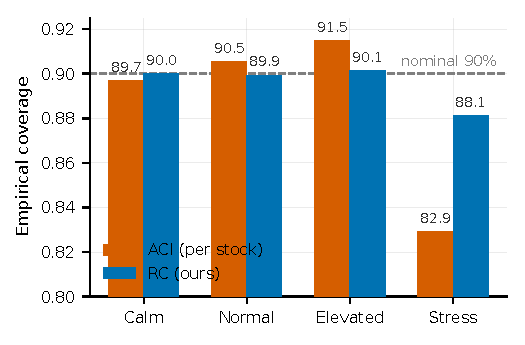
\includegraphics{figures/fig_coverage_by_regime.pdf}
\caption{Coverage of nominal 90\% intervals by market regime, 2010--2025
(269{,}705 common stock-days). Per-stock ACI is marginally valid (89.9\%)
but redistributes its errors: over-coverage in elevated regimes pays for
82.9\% coverage in stress. The regime-conditional layer (RC) removes most
of the conditional deficit while holding other regimes at nominal.}
\label{fig:coverage}
\end{figure}

Table~\ref{tab:main} is the paper's central comparison: thirteen methods
on the identical common sample. The baselines span the online conformal
family (ACI, DtACI, SF-OGD), conformal PID control
\citep{angelopoulos2023conformal} (quantile tracking, saturated
integrator, and a trailing-quantile scorecaster, per stock --- the
method whose integrator structure our corrector borrows), the recent
rolling-conformal method of
\citet{aich2025temporal} with its Robbins--Monro coverage offset (TCP-RM,
ported to our score scale with its published constants), a classical
direct-quantile model (HAR quantile regression), a similarity-weighted
conformal method (KNN-state, in the spirit of HopCPT/NexCP: thresholds
from the $k = 250$ most similar past days by market state), a
cross-sectional split-conformal baseline in the spirit of
\citet{wtqa2026panel} (XS-panel: each day's thresholds from the pooled
score cross-sections of the previous five days, with an adaptive
miscoverage level; their contemporaneous-outcome construction is not
available when all next-day forecasts are issued simultaneously, so this
is an adaptation to our information structure, not the original
algorithm), and two group-conditional methods handed our own hard VIX
bins as their groups --- the exact interface their guarantees require:
the parameter-free coin-betting method of
\citet{bharti2026parameterfree} (POGO, per stock as its single-stream
setting specifies) and the no-regret FTRL scheme of
\citet{ramalingam2025noregret} (RKR, per stock, with overlapping
marginal-plus-bin groups). Comparator constants were fixed once, from
each source paper's own conventions or data requirements, and not
revisited; the one comparator setting the conclusions are sensitive to
--- the adaptive rate-grid ceiling --- is swept explicitly in
Table~\ref{tab:expgrid}. Every marginal coverage sits
within half a point of 90\%; every baseline's stress coverage sits between
81.5\% and 84.9\%. The two regime-conditional variants (hand-tuned
rates and the zero-tuning adaptive configuration) reach 88.1--88.2\%,
with the stress upper tail at 94.0\% against 95\% nominal versus
84.8--91.0\% for the baselines. These differences carry real
uncertainty, and we quantify it two ways, matched to where the
dependence lives. First, \emph{date-clustered HAC}: coverage indicators
are averaged within each date (removing all cross-sectional dependence),
and the resulting daily series --- for stress slices, the 150 stress
dates in event time --- gets a Newey--West variance with Bartlett kernel
and the $\lfloor 4(n/100)^{2/9} \rfloor$ lag rule (lag 4 here); reported
$\pm$ values are one standard error. Stress coverage is
$.881 \pm .019$ for RC against $.830 \pm .026$ for ACI; the paired
stress-coverage difference is $+5.1$ points against ACI ($t = 3.05$,
$p = .002$, stable for lags 0--22 and $p = .07$ at lag 66), significant
at the 1\% level against every per-stock baseline except TCP-RM ($+3.1$
points, $p = .027$), while marginal coverage differences among the
conformal methods are statistically zero ($|t| < 0.5$), exactly as
marginal validity predicts. Second, and more conservatively,
\emph{episode-block resampling}: stress days group into 18 contiguous
episodes (gaps above 20 trading days), and resampling episodes with
replacement (10{,}000 draws) gives $+5.2$ points against ACI with a
95\% interval of $[-0.1, +9.7]$ ($p = .057$). The widening is not an
artifact: the gap genuinely differs across episodes --- large in the
fast shifts of 2018--2025, absent to slightly negative before
(Table~\ref{tab:temporal}) --- and 18 episodes is all the
twenty-one-year sample contains. Against XS-panel, whose deficit is
uniform across eras, the episode-resampled interval excludes zero
($[+2.8, +8.9]$, $p < .001$). Both inferential treatments are reported: the repair is
era-dependent insurance, large when fast regime shifts occur and
approximately free when they do not.

Because the comparisons above are many --- thirteen methods, four
regimes, two tails, two eras --- we prespecify one \emph{primary
endpoint} and treat everything else as secondary. The primary endpoint
is the stress-day \emph{upper-tail} coverage difference against ACI,
the direction that maps to risk losses, estimated on the full calendar
(not event time) by regressing the daily paired difference on a stress
indicator: the calm-day gap is $-0.1$ points (as it should be) and the
stress increment is $+4.0$ points, significant under calendar-time HAC
($p = .009$), under episode-clustered standard errors ($p = .016$), and
under a wild cluster bootstrap over the 18 episodes ($p = .003$), with
leave-one-episode-out estimates spanning $[+2.3, +4.8]$ --- always
positive. The secondary two-sided stress increments are positive
against every per-stock baseline ($+3.3$ to $+5.8$ points, calm gaps
$\approx 0$) but individually weaker under episode-level wild
bootstrap ($p = .13$--$.34$), and a Romano--Wolf stepdown across all
baselines leaves only the POGO and XS-panel comparisons significant
after multiplicity adjustment (adjusted $p = .017$ and $.041$; ACI
adjusted $p = .099$). We state the resulting evidential hierarchy
explicitly: the upper-tail repair is certified under the most
conservative treatment we know how to run; the two-sided secondary
gaps are consistent in sign and era-concentrated but not individually
certified against episode-level variation. Efficiency admits a formal
non-inferiority statement: the paired daily interval-score difference
against ACI is $-0.003$ with 95\% interval $[-0.022, +0.015]$, inside
a prespecified margin of 2\% of ACI's mean score, so RC is
statistically non-inferior on average efficiency, not merely
``no detected loss.''

Because the guarantee is panel-level (Remark~\ref{rem:panel}), a pooled
threshold could in principle hide stock-level failures behind a valid
regime average. Table~\ref{tab:perstock} shows it does the opposite:
pooling lifts the \emph{entire} cross-sectional distribution of
stock-level stress coverage. The median stock moves from 83.9\% to
88.0\%, the worst decile from 78.0\% to 84.6\%, and the share of stocks
below 85\% stress coverage falls from 70\% to 14\%.

\begin{table}[t]
\centering
\caption{Per-stock coverage distribution, common sample, stocks
with at least 25 stress observations ($n = 107$; marginal rows use all
136 stocks). Quantiles of realized per-stock coverage of nominal 90\%
intervals.}
\label{tab:perstock}
\small
\begin{tabular}{llccccc}
\toprule
 & & q05 & q10 & Median & q75 & Share $<$ .85 \\
\midrule
Marginal & ACI & .885 & .891 & .898 & .900 & .00 \\
 & RC (adaptive) & .883 & .885 & .899 & .906 & .00 \\
\addlinespace
Stress & ACI & .757 & .780 & .839 & .859 & .70 \\
 & RC (adaptive) & \textbf{.834} & \textbf{.846} & \textbf{.880} & \textbf{.900} & \textbf{.14} \\
\bottomrule
\end{tabular}
\end{table}

\begin{table}[t]
\centering
\caption{Main comparison: coverage of nominal 90\% intervals and
interval widths on the common sample. ``Stress up'' is upper-tail coverage
in stress (nominal 95\%). RC~=~regime-conditional pooled layer.}
\label{tab:main}
\small
\begin{tabular}{lcccccc}
\toprule
 & Marginal & Calm & Stress & Stress up & Width & Width (stress) \\
\midrule
ACI & .899 & .897 & .829 & .901 & 1.70 & 1.80 \\
DtACI & .899 & .897 & .836 & .906 & 1.70 & 1.87 \\
SF-OGD & .899 & .898 & .840 & .910 & 1.73 & 1.91 \\
TCP-RM & .900 & .899 & .849 & .919 & 1.79 & 2.07 \\
CPID & .899 & .898 & .836 & .905 & 1.72 & 1.85 \\
RKR & .898 & .900 & .846 & .918 & 1.72 & 1.92 \\
HAR-QREG & .890 & .886 & .815 & .848 & 1.65 & 1.71 \\
KNN-state & .894 & .892 & .829 & .908 & 1.67 & 1.84 \\
XS-panel & .900 & .907 & .827 & .933 & 1.80 & 1.99 \\
POGO & .858 & .871 & .771 & .885 & 1.74 & 2.14 \\
Pooled, $K=1$ (no regimes) & .900 & .901 & .873 & .941 & 1.73 & 2.27 \\
RC (hand-tuned) & .898 & .899 & \textbf{.882} & \textbf{.941} & 1.70 & 2.25 \\
RC (adaptive) & .899 & .900 & \textbf{.881} & \textbf{.940} & 1.73 & 2.34 \\
\bottomrule
\end{tabular}
\end{table}

Six readings of Table~\ref{tab:main} matter. First, pooling without
regimes already does most of the average work: the pooled $K = 1$ row
reaches 87.3\% stress coverage, and the regime layer's further average
contribution is $+0.8$ points (not significant under date clustering,
$t = 0.6$); what regimes buy instead is conditional structure,
quantified in Section~\ref{sec:ablations}. Second, the repair is a
\emph{reallocation}, not an inflation: RC average width matches ACI (1.73
vs 1.70) because width moves into stress ($+$30\%) and out of regimes
where baselines over-cover. Third, the reallocation is not detectably
costly by the standard efficiency metric of the interval-forecasting
literature: a Model Confidence Set \citep{hansen2011model}
over daily cross-sectional mean interval scores \citep{winkler1972decision}
retains both RC variants among the undominated set (RC hand-tuned has the
lowest mean loss) and eliminates SF-OGD, TCP-RM, CPID, RKR, XS-panel,
and POGO ($p \le .001$); we do not detect inferior average
interval-score performance. Fourth, similarity weighting
without a coverage feedback loop does not solve the problem: KNN-state
improves on ACI in stress by only 0.1 points. Selecting similar days is
not the same as tracking a coverage target within a regime, which is why our
pooling operates inside the tracking loop. Fifth, the recently proposed baselines bracket our design and fall
short from different directions. TCP-RM is the strongest per-stock
method in stress (84.9\%, still $3.1$ points below RC, $t = 2.21$,
$p = .027$, the only pairwise gap outside the 1\% level) but pays for
it with the widest per-stock intervals, because its rolling 60-day
window forgets calm-period scores wholesale rather than conditioning on
the regime. RKR --- the no-regret multigroup generalization of ACI,
given our bins --- is next at 84.6\% ($-3.5$, $p = .007$): the
group-conditional update helps a single stream, but a stock's own
stress history remains too short. Conformal PID reaches 83.6\%
($-4.3$, $p = .008$), which matters for mechanism attribution: our
corrector borrows PID's integrator structure, so the gain over CPID is
not ``PID plus a faster rate'' --- it is the pooled panel signal that
integrator consumes. XS-panel
calibrates on recent cross-sections of the same panel our method pools
(the most recent five observed days; the original method's
contemporaneous-outcome construction is not available when all next-day
forecasts are issued simultaneously), yet its stress coverage (82.7\%)
is indistinguishable from ACI's: recent cross-sections tell the
calibrator how wide intervals should be, but without per-regime tracking
the adaptive level still reacts only after misses accumulate.
Cross-sectional information and coverage feedback each fail separately;
the gain comes from combining them inside regime-conditional trackers.
Sixth, a published group-conditional guarantee is not the same as
delivered conditional coverage: POGO, handed our own regime bins as its
groups, covers 85.8\% marginally and 77.1\% in stress ($-11.0$ points
against RC, $t = 8.4$). The
realized coverage is consistent with its stated parameter-free bound,
which at a per-stock horizon of $T \approx 3{,}800$ rounds permits
per-side slack of roughly 2.5 points and is vacuous for a 150-round
stress group. It is evidence that at equity-panel sample sizes the group
interface alone does not bite; the coverage must come from the tracking
loop, which is what the pooled per-observation update supplies.

\subsection{Self-tuning rates}\label{sec:adaptive}

The adaptive configuration replaces every hand-chosen learning rate with
per-regime expert aggregation plus the issued-interval corrector
(Section~\ref{sec:method}). With no hand-tuned learning rates it ties the
hand-tuned stress coverage (88.1 vs 88.2), improves calm/normal coverage
to 90.0, and costs 2\% average width. Its learned effective rates
recover, online, both regularities that manual tuning had discovered:
stress-regime effective rates converge to $\approx 0.009$ against a
hand-tuned $0.01$, and 1\%-VaR rates to $\approx 0.020$ against a
hand-tuned $0.02$. We treat the adaptive configuration as the headline
method and the hand-tuned one as an ablation.

\subsection{Value-at-Risk}\label{sec:var}

\begin{figure}[t]
\centering
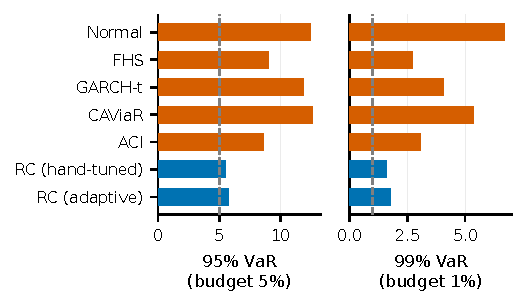
\includegraphics{figures/fig_var_breach.pdf}
\caption{Stress-day VaR breach rates against the nominal budgets
(dashed). Classical parametric models and per-stock conformal baselines
alike breach two to six times their budget on stress days; the pooled
heads come closest to nominal, and among them only the
regime-conditional head balances calm and stress
(Table~\ref{tab:var}).}
\label{fig:var}
\end{figure}

Table~\ref{tab:var} and Figure~\ref{fig:var} apply the one-sided head
to next-day VaR and backtest all methods per stock with the Kupiec
unconditional-coverage test, the Christoffersen \emph{independence}
test, their combined conditional-coverage (CC) test, and the
Engle--Manganelli dynamic-quantile test augmented with a stress-regime
indicator regressor (DQ-S), all at 5\% significance; tests run over
each stock's full evaluation sequence. The classical parametric models
fail exactly where the conformal baselines do: on stress days, 99\% VaR
breach rates are 4.1\% (GARCH-$t$), 5.4\% (CAViaR), and 3.1\% (ACI)
against a 1\% budget. The RC head reaches 1.8\% (still above nominal,
and we say so) with marginal rates of 5.00/1.07 against 5/1 budgets.
Conditional balance is where the regime layer is statistically
unambiguous: a date-clustered test of equal calm and stress exceedance
rates at the 5\% level rejects for every baseline (all overshoot
stress, $z = 2.1$ to $3.9$) and for the pooled $K = 1$ head in the
\emph{opposite} direction (calm 5.3\% vs.\ stress 3.7\%, $z = -1.8$);
only the regime-conditional heads are balanced (5.0/5.7, $z = 0.5$). At
the deep 1\% tail the ordering partially reverses: pooled $K = 1$ posts
the best CC and DQ-S pass shares (.91/.73 against RC's .87/.64),
consistent with the data-splitting cost of conditioning noted in
Section~\ref{sec:ablations}; we report both levels rather than average
over them.

\begin{table}[t]
\centering
\caption{Next-day VaR backtests. Stress-day breach rates against
nominal budgets of 5\% and 1\%; ``Balance $z$'' tests equality of calm
and stress exceedance rates at the 5\% level (date-clustered; positive
means stress overshoots). The last three columns are the shares of
stocks whose 99\% VaR sequence passes the Kupiec, combined
conditional-coverage (CC), and stress-augmented dynamic-quantile (DQ-S)
tests at 5\% significance. Christoffersen independence pass shares are
.79--.97 for all methods and are reported in the replication
artifacts.}
\label{tab:var}
\small
\begin{tabular}{lcccccc}
\toprule
 & \multicolumn{2}{c}{Stress breach rate} & &
   \multicolumn{3}{c}{99\% VaR pass shares} \\
\cmidrule(lr){2-3} \cmidrule(lr){5-7}
 & 95\% VaR & 99\% VaR & Balance $z$ & Kupiec & CC & DQ-S \\
\midrule
Normal (Gaussian) & 12.5\% & 6.7\% & $+$2.6 & .05 & .05 & .01 \\
FHS & 9.0\% & 2.7\% & $+$2.2 & .88 & .83 & .52 \\
GARCH-$t$ & 11.9\% & 4.1\% & $+$3.5 & .56 & .63 & .27 \\
CAViaR & 12.6\% & 5.4\% & $+$3.9 & .52 & .56 & .23 \\
ACI & 8.6\% & 3.1\% & $+$2.1 & .60 & .60 & .36 \\
Pooled $K=1$ & 3.7\% & \textbf{1.2\%} & $-$1.8 & .83 & \textbf{.91} & \textbf{.73} \\
RC (hand-tuned) & 5.5\% & 1.6\% & $+$0.3 & .83 & .84 & .61 \\
RC (adaptive) & \textbf{5.7\%} & 1.8\% & $\mathbf{+0.5}$ & \textbf{.88} & .87 & .64 \\
\bottomrule
\end{tabular}
\end{table}

\subsection{The same failure in a time-series foundation model}\label{sec:tsfm}

\begin{figure}[t]
\centering
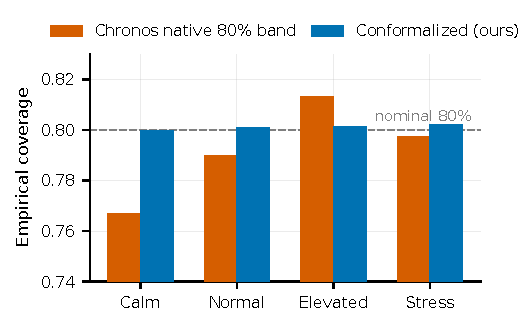
\includegraphics{figures/fig_tsfm_repair.pdf}
\caption{Chronos-Bolt's native 80\% band by regime, before and after
conformalization. The native band under-covers everywhere except the
elevated regime, and its stress misses are concentrated on the upside
(14.6\% against a 10\% budget); the conformal layer flattens coverage to
80.0--80.2\% across regimes.}
\label{fig:tsfm}
\end{figure}

Chronos-Bolt (the \texttt{amazon/chronos-bolt-small} checkpoint, 48M
parameters), applied zero-shot to each stock's
trailing 512-day log-RV history \citep{ansari2024chronos}, is competitive on point accuracy with no
training, consistent with \citet{brini2026forecasting}, but its
native 80\% band covers 77.9\% marginally and is \emph{directionally}
wrong in stress: 14.6\% upside misses against a 10\% budget versus 5.7\%
downside, so the stress miss asymmetry is concentrated on the side that
matters for risk. The official checkpoint outputs nine quantiles from
0.1 to 0.9, capping any native risk use; whether the asymmetry reflects
uncertainty-scale failure or point-location bias in the median is not
separable at this quantile resolution. Constructing regime-calibrated intervals around Chronos's median with our
layer flattens coverage to 80.0--80.2\% across regimes
(Figure~\ref{fig:tsfm}). The repair is
forecaster-agnostic by construction; this experiment shows it extends to
the model class currently entering forecasting practice.

\subsection{Crisis episodes, holdout, and robustness}\label{sec:episodes}

A conditioning-scheme referee should also ask whether the evaluation is
self-referential: the algorithm conditions on VIX-percentile bins and
the canonical stress slice uses the same partition. Re-slicing the
identical issued intervals by stress definitions \emph{external} to
the algorithm answers this. The RC--ACI gap survives every acute
volatility definition --- absolute VIX $\ge 30$ ($+2.7$ points,
$p = .015$, 230 dates), market realized-volatility tail ($+4.1$,
$p = .003$), the eight named crisis windows ($+1.3$, $p = .06$) ---
and attenuates, as it mechanically must, on broad definitions
dominated by moderate-volatility days where ACI is already adequate
(absolute VIX $\ge 25$: $+0.5$, n.s.) or on stress notions that are
not acute-volatility events at all (credit-spread tail: $+0.7$,
n.s.). The repair is a property of acute volatility states however
defined, not of the VIX-percentile encoding.

\begin{figure}[t]
\centering
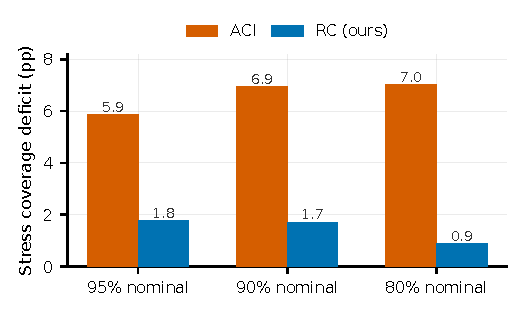
\includegraphics{figures/fig_alpha_sweep.pdf}
\caption{Stress coverage deficit (percentage points below the nominal
level) across nominal levels. The conditional failure and its repair
are not artifacts of the 90\% level.}
\label{fig:alpha}
\end{figure}

\begin{figure}[t]
\centering
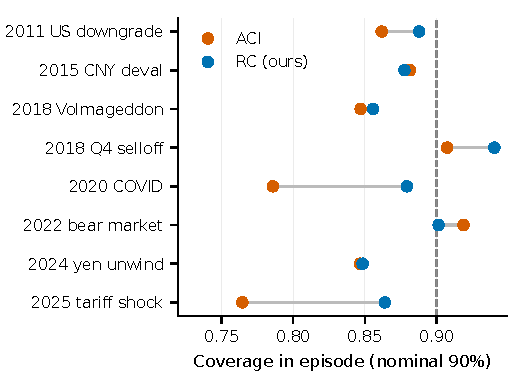
\includegraphics{figures/fig_episodes.pdf}
\caption{Coverage of nominal 90\% intervals within eight crisis episodes
RC improves the four worst episodes, with COVID up 9.3 points
(.786 $\to$ .879) and the 2025 tariff shock up 9.7 (.765 $\to$ .862),
and tracks nominal more closely in episodes where ACI over-covers (2022).
Flash-onset episodes (2015, 2024) move least, consistent with
Section~\ref{sec:onset}.}
\label{fig:episodes}
\end{figure}

Figure~\ref{fig:episodes} slices the sample into eight named stress
windows. The pattern is the day-2 result writ large: episodes with
sustained stress (COVID, 2018~Q4, 2011, 2025) improve by 3--10 points;
one-week flash events dominated by their onset days (2015 CNY devaluation,
2024 yen unwind) barely move: the same onset boundary. Robustness
checks (artifacts in the replication package): the failure and its repair
reproduce on disjoint alternating-alphabet halves of the universe with a
frozen configuration (stress coverage .832/.829 ACI vs .875/.876 RC);
conclusions are stable across $\alpha \in \{0.05, 0.10, 0.20\}$, where the
stress coverage deficit stays near 6--7 points for ACI and 1--2 points for
RC at every level (Figure~\ref{fig:alpha}); and replacing
VIX bins with the online HMM changes stress coverage by under two points,
so no conclusion depends on the regime estimator.

Time is the other axis a design could overfit. Every constant in the
method is fixed a priori (\ref{app:algorithm}) and calibration is
fully online, so there is no fitting step to freeze; the temporal question
is whether the conclusions depend on any particular stretch of the
evaluation window. Table~\ref{tab:temporal} splits the evaluation at
January 2018. The stress deficit turns out to be a phenomenon of the
recent market era: in 2010--2017 (whose stress episodes, 2011 and 2015,
built up comparatively slowly) ACI's stress coverage was adequate at
89.6\%, while in 2018--2025 (Volmageddon, COVID, the 2022 bear market,
the 2024 yen unwind, the 2025 tariff shock) it collapses to 78.8\%. RC
delivers 88.3\% in \emph{both} halves: the paired stress gap is $+9.4$
points ($t = 4.3$) in the second half and $-1.3$ points (not significant,
$p = .06$) in the first. The method behaves like insurance: large payoff
in the era of fast regime shifts, no significant cost in the era without
them. Leave-one-crisis-out slicing shows the same stability: dropping any single episode's stress days moves RC stress
coverage by at most 0.4 points (range .881--.887), while ACI stays
deficient no matter which crisis is removed (at most .854, with COVID
excluded).

\begin{table}[t]
\centering
\caption{Temporal robustness: the same issued intervals evaluated
by subperiod, full panel. The paired stress gap is the date-clustered
difference RC~$-$~ACI on common stress days.}
\label{tab:temporal}
\small
\begin{tabular}{llcccc}
\toprule
Period & Method & Marginal & Stress & Stress up & Stress gap ($t$) \\
\midrule
2010--2017 & ACI & .898 & .896 & .927 & \\
 & RC (adaptive) & .898 & .883 & .932 & $-1.3$ ($-1.9$) \\
\addlinespace
2018--2025 & ACI & .899 & .788 & .881 & \\
 & RC (adaptive) & .900 & .883 & .944 & $+9.4$ ($4.3$) \\
\bottomrule
\end{tabular}
\end{table}
